\documentclass[11pt,a4paper]{article}
\usepackage[utf8]{inputenc}
\usepackage{amsmath, amssymb}
\usepackage{graphicx}
\usepackage{booktabs}
\usepackage{geometry}
\usepackage{caption}
\usepackage{subcaption}
\usepackage{hyperref}
\usepackage{listings}
\usepackage{xcolor}
\geometry{margin=2.5cm}

% MATLAB listing style
\lstdefinestyle{matlab}{
    language=Matlab,
    basicstyle=\ttfamily\footnotesize,
    keywordstyle=\color{blue},
    commentstyle=\color{green!50!black},
    stringstyle=\color{red},
    numbers=left,
    numberstyle=\tiny\color{gray},
    frame=single,
    breaklines=true,
    captionpos=b
}

\title{Classification of Iris Flowers and Handwritten Digits \\[0.5em]
\large TTT4275 Estimation, Detection and Classification --- NTNU}
\author{Student A \and Student B}
\date{\today}

\begin{document}
\maketitle

%% ======================================================================
%% SUMMARY
%% ======================================================================
\begin{abstract}
This report presents the two classification projects assigned in TTT4275. The first project is the mandatory Iris task, in which a linear classifier is trained by minimizing the mean squared error (MSE) via iterative gradient descent. The effect of the training/test split on generalization is investigated, and the relative importance of the four features is analysed by progressively removing the least discriminative feature. The second project addresses classification of handwritten digits from the MNIST database using variants of the nearest-neighbour classifier described in chapter~3 of the course compendium. A 1-NN classifier built from all 60\,000 training images is compared with 1-NN and 7-NN classifiers built from a compact template set produced by per-class $k$-means clustering. Both projects follow the constructions given in the compendium, and the code is provided in the appendices.
\end{abstract}

\tableofcontents
\newpage

%% ======================================================================
\section{Introduction}
%% ======================================================================

Pattern classification is a central problem in signal processing and machine learning, where the goal is to assign an observation to one of several predefined categories based on measured features. It has broad applications ranging from medical diagnosis to speech recognition and autonomous systems.

This report covers the two classification projects assigned in TTT4275. The first is the Iris task, which uses the classical Fisher Iris dataset~\cite{fisher1936} of 150 flower samples from three species described by four measurements each. The dataset is close to linearly separable and is used to train and evaluate the linear MSE classifier of chapters~2.4--3.2 of the compendium~\cite{compendium}. The second project is the MNIST handwritten-digit classification task. Here a $28\!\times\!28$-pixel image is treated as a 784-dimensional feature vector and classified with the nearest-neighbour (NN) and $K$-nearest-neighbour (KNN) classifiers of chapter~3, applied both to the full 60\,000-image training set and to a compact template set obtained by per-class $k$-means clustering.

The rest of this report is organized as follows. Section~\ref{sec:theory} presents the theoretical background on the linear MSE classifier and the nearest-neighbour classifiers used later. Section~\ref{sec:task} describes the specific tasks. Section~\ref{sec:iris_results} covers the Iris implementation and results, and Section~\ref{sec:mnist_results} covers the MNIST implementation and results. Section~\ref{sec:conclusion} summarizes the main findings.

%% ======================================================================
\section{Theory}
\label{sec:theory}
%% ======================================================================

This section presents the theory behind the linear MSE classifier used in this project. The derivations follow the course compendium~\cite{compendium}, chapters~2.4 and~3.2.

\subsection{Linear Discriminant}

A linear discriminant classifier describes each class $\omega_i$ by a linear function (compendium Eq.~7)
\begin{equation}
    g_i(\mathbf{x}) = \mathbf{w}_i^T \mathbf{x} + w_{i0}, \qquad i = 1,\dots,C.
    \label{eq:discriminant}
\end{equation}
Stacking the bias into the weight matrix $\mathbf{W} \in \mathbb{R}^{C \times (D+1)}$ and augmenting the feature vector as $\tilde{\mathbf{x}} = [\mathbf{x}^T\; 1]^T$ gives the compact form $\mathbf{z} = \mathbf{W}\tilde{\mathbf{x}}$. A sample $\mathbf{x}$ is assigned to the class $\hat{c}$ corresponding to the largest discriminant value (Eq.~6):
\begin{equation}
    \hat{c} = \arg\max_{i}\; g_i(\mathbf{x}).
    \label{eq:classification}
\end{equation}

\subsection{Sigmoid Activation}

Since the one-hot targets take binary values $\{0,1\}$, the raw discriminant $\mathbf{z} = \mathbf{W}\tilde{\mathbf{x}}$ is passed through a smooth sigmoid (compendium Eq.~20):
\begin{equation}
    g_{ik} \;=\; \mathrm{sigmoid}(z_{ik}) \;=\; \frac{1}{1+e^{-z_{ik}}}, \qquad i=1,\dots,C.
    \label{eq:sigmoid}
\end{equation}
The sigmoid is used because the gradient-descent training in the next subsection requires a differentiable approximation of the Heaviside step; since it is monotonic, it does not change the argmax decision in Eq.~\eqref{eq:classification}.

\subsection{MSE Training Criterion}

The weight matrix $\mathbf{W}$ is found by minimizing the mean squared error between the classifier outputs and the one-hot targets $\mathbf{t}_k \in \{0,1\}^C$ (compendium Eq.~19):
\begin{equation}
    \mathrm{MSE} \;=\; \tfrac{1}{2}\sum_{k=1}^{N} \bigl(\mathbf{g}_k - \mathbf{t}_k\bigr)^T \bigl(\mathbf{g}_k - \mathbf{t}_k\bigr).
    \label{eq:mse}
\end{equation}

\subsection{Gradient and Update}

Because the sigmoid is smooth, the gradient of the MSE in Eq.~\eqref{eq:mse} can be obtained through the chain rule. Using $\nabla_{\mathbf{g}_k}\mathrm{MSE} = \mathbf{g}_k - \mathbf{t}_k$, the sigmoid derivative $\nabla_{\mathbf{z}_k}\mathbf{g}_k = \mathbf{g}_k \circ (\mathbf{1}-\mathbf{g}_k)$ and $\nabla_{\mathbf{W}}\mathbf{z}_k = \mathbf{x}_k^T$, one obtains (compendium Eq.~22):
\begin{equation}
    \nabla_{\mathbf{W}} \mathrm{MSE}
    \;=\; \sum_{k=1}^{N}
    \bigl[(\mathbf{g}_k - \mathbf{t}_k)\circ \mathbf{g}_k \circ (\mathbf{1} - \mathbf{g}_k)\bigr]\,\mathbf{x}_k^T,
    \label{eq:gradient}
\end{equation}
where $\circ$ denotes elementwise multiplication. The weights are updated in the opposite direction of the gradient (compendium Eq.~23):
\begin{equation}
    \mathbf{W}(m) \;=\; \mathbf{W}(m-1) - \alpha\,\nabla_{\mathbf{W}} \mathrm{MSE},
    \label{eq:update}
\end{equation}
where $\alpha > 0$ is the step factor, which is chosen by trial and error so that the MSE decreases monotonically without oscillating.

\subsection{Nearest-Neighbour and K-Nearest-Neighbour Classifiers}
\label{subsec:nn_theory}

The compendium describes in chapter~3 a complementary family of classifiers that do not estimate a parametric decision surface but store a set of labelled reference vectors (``templates'') $\{\mathbf{t}_j, c_j\}_{j=1}^{N_T}$. For a new sample $\mathbf{x}$ the Euclidean distance
\begin{equation}
    d(\mathbf{x}, \mathbf{t}_j) \;=\; \|\mathbf{x} - \mathbf{t}_j\|_2
    \;=\; \sqrt{(\mathbf{x} - \mathbf{t}_j)^T(\mathbf{x} - \mathbf{t}_j)}
    \label{eq:euclidean}
\end{equation}
is computed to every template, and the \emph{nearest-neighbour} (NN) rule assigns the class of the closest template:
\begin{equation}
    \hat{c}_\text{NN}(\mathbf{x}) \;=\; c_{j^\star}, \qquad
    j^\star = \arg\min_{j}\; d(\mathbf{x}, \mathbf{t}_j).
    \label{eq:nn}
\end{equation}
The \emph{$K$-nearest-neighbour} (KNN) rule is a robust generalization: the $K$ closest templates $\{\mathbf{t}_{j_1},\dots,\mathbf{t}_{j_K}\}$ are located and $\mathbf{x}$ is assigned to the class that occurs most frequently among their labels:
\begin{equation}
    \hat{c}_\text{KNN}(\mathbf{x}) \;=\; \mathrm{mode}\bigl(c_{j_1},\dots,c_{j_K}\bigr).
    \label{eq:knn}
\end{equation}
When $N_T$ is very large (60\,000 MNIST images) the classifier is slow because the full $N_\text{test}\times N_T$ distance matrix must be evaluated. For computational efficiency the distances are computed in chunks using the identity
\begin{equation}
    \|\mathbf{x}-\mathbf{t}\|_2^2 \;=\; \|\mathbf{x}\|_2^2 + \|\mathbf{t}\|_2^2 - 2\,\mathbf{x}^T\mathbf{t},
    \label{eq:dist_trick}
\end{equation}
so that the cross-term reduces to a single matrix product.

\subsection{Template Clustering}
\label{subsec:kmeans}

The KNN classifier can be made faster and more robust by replacing the 60\,000 training images with a small set of \emph{prototypes} found by clustering. For each class $\omega_i$ separately, the training vectors are grouped into $M$ clusters by $k$-means, which iteratively minimizes the within-cluster sum of squares
\begin{equation}
    J \;=\; \sum_{m=1}^{M} \sum_{\mathbf{x}_k \in \mathcal{S}_m} \|\mathbf{x}_k - \mathbf{c}_m\|_2^2,
    \label{eq:kmeans}
\end{equation}
where $\mathcal{S}_m$ is the set of training vectors assigned to cluster $m$ and $\mathbf{c}_m$ is the corresponding centroid. The $C\cdot M$ centroids are then used as templates in Eqs.~\eqref{eq:nn}/\eqref{eq:knn}.

\subsection{Confusion Matrix and Error Rate}

Classifier performance is evaluated using a confusion matrix, which is a $C \times C$ matrix where element $(i,j)$ counts the number of samples from true class $i$ that were classified as class $j$. The overall error rate is defined as
\begin{equation}
    \text{Error rate} = \frac{\text{Number of misclassified samples}}{\text{Total number of samples}} \times 100\%.
    \label{eq:errorrate}
\end{equation}

%% ======================================================================
\section{The Task}
\label{sec:task}
%% ======================================================================

This section describes the tasks addressed in this report. The project assignment offers a choice between multiple classification problems; the Iris task is mandatory for all groups, and we have additionally chosen the MNIST handwritten-digit task.

\subsection*{Iris}
The Iris dataset contains 50~samples from each of three flower species (Setosa, Versicolor, Virginica), with four features per sample (sepal length, sepal width, petal length, petal width). Two sub-tasks are performed:

\textbf{Task~1 --- Training and generalization.} A linear MSE classifier is trained and tested using two different train/test splits: first using the first 30~samples per class for training and the last 20 for testing, then swapping so that the last 30 are used for training and the first 20 for testing. Confusion matrices and error rates are computed for both the training and test sets in each case, and the results are compared.

\textbf{Task~2 --- Features and linear separability.} Using the first train/test split from Task~1, histograms of each feature are plotted per class. The feature showing the most overlap between classes is identified and removed. The classifier is then retrained and tested with the remaining three features. This process is repeated, removing one more feature at each step, resulting in classifiers using 4, 3, 2, and 1 features. The confusion matrices and error rates are compared to assess the relative importance of each feature for linear separability.

\subsection*{MNIST}
The MNIST database contains 60\,000 training images and 10\,000 test images of handwritten digits $0$--$9$, each a $28\!\times\!28$-pixel 8-bit grayscale image ($784$-dimensional feature vector). Two sub-tasks are performed using the nearest-neighbour classifiers of Section~\ref{subsec:nn_theory}.

\textbf{Task~1 --- NN classifier with the full template set.} A 1-NN classifier using all 60\,000 training images as templates is designed. The test set is processed in chunks of 1000 images to keep the distance matrix tractable. Confusion matrix, error rate and examples of correctly and incorrectly classified images are produced.

\textbf{Task~2 --- Cluster templates, NN and KNN.} The training vectors of each class are clustered into $M=64$ prototypes with $k$-means, giving a total of $640$ templates. A 1-NN classifier is built on these templates, and then a KNN classifier with $K=7$. Processing time and performance are compared to the full-template classifier.

%% ======================================================================
\section{Iris --- Implementation and Results}
\label{sec:iris_results}
%% ======================================================================

This section describes how the Iris linear classifier was implemented in MATLAB and presents the results for both sub-tasks. The full MATLAB code is provided in Appendix~\ref{app:iris_code}.

\subsection{Implementation Overview}

The Iris dataset is provided as three separate ASCII files (\texttt{class\_1}, \texttt{class\_2}, \texttt{class\_3}), one per species, each containing 50 samples with four comma-separated feature values. The data is loaded with \texttt{load('class\_1','-ascii')} and analogously for the other two classes, yielding three $50 \times 4$ matrices. One-hot target vectors $\mathbf{t}_k$ are built by assigning a 1 to the column corresponding to the true class.

The feature vectors are augmented with a trailing 1 to absorb the bias $w_{i0}$ into $\mathbf{W}$. The weight matrix is initialized with small random values ($\sim\!\mathcal{N}(0,10^{-2})$). In each gradient-descent iteration the code evaluates, in this order, the discriminant $\mathbf{z}=\mathbf{W}\tilde{\mathbf{x}}$, the sigmoid activation of Eq.~\eqref{eq:sigmoid}, the MSE of Eq.~\eqref{eq:mse}, the gradient of Eq.~\eqref{eq:gradient}, and the weight update of Eq.~\eqref{eq:update}. The step factor was tuned by trial and error to $\alpha = 0.005$; with this value, $M = 3000$ batch iterations are sufficient for the MSE to flatten out. After training, each sample is classified with Eq.~\eqref{eq:classification} (argmax of the sigmoid outputs, equivalent to argmax of $\mathbf{z}$ since the sigmoid is monotone). The $C \times C$ confusion matrix is built by counting, for each true class $i$, how many samples the classifier assigned to class $j$.

Figure~\ref{fig:flowchart} illustrates the overall training and evaluation procedure.

\begin{figure}[ht]
\centering
\fbox{\parbox{0.85\textwidth}{\centering
\textbf{Flow diagram:} \\[0.5em]
Load data $\rightarrow$ Split into train/test $\rightarrow$ Augment features $\rightarrow$ Initialize $\mathbf{W}$ $\rightarrow$ \\
Gradient descent loop (5000 iterations) $\rightarrow$ \\
Classify train \& test sets $\rightarrow$ Compute confusion matrices \& error rates
}}
\caption{Overview of the training and evaluation pipeline.}
\label{fig:flowchart}
\end{figure}

\subsection{Task 1: Training and Generalization}

\textbf{Case~1} uses the first 30 samples per class for training (90 total) and the last 20 for testing (60 total). \textbf{Case~2} reverses this split. The training MSE (Eq.~\eqref{eq:mse}) was monitored for each iteration and converged smoothly to a stable plateau in both cases (see \texttt{mse\_case1.png} and \texttt{mse\_case2.png} produced by the script).

\bigskip
\noindent\textbf{Case 1 --- Training confusion matrix:}
\begin{center}
\begin{tabular}{c|ccc}
\toprule
 & Pred.\ Setosa & Pred.\ Versicolor & Pred.\ Virginica \\
\midrule
Setosa     & 30 & 0  & 0  \\
Versicolor & 0  & 28 & 2  \\
Virginica  & 0  & 1  & 29 \\
\bottomrule
\end{tabular}
\end{center}
Training error rate: $3/90 = 3.33\,\%$.

\bigskip
\noindent\textbf{Case 1 --- Test confusion matrix:}
\begin{center}
\begin{tabular}{c|ccc}
\toprule
 & Pred.\ Setosa & Pred.\ Versicolor & Pred.\ Virginica \\
\midrule
Setosa     & 20 & 0  & 0  \\
Versicolor & 0  & 18 & 2  \\
Virginica  & 0  & 0  & 20 \\
\bottomrule
\end{tabular}
\end{center}
Test error rate: $2/60 = 3.33\,\%$.

\bigskip
\noindent\textbf{Case 2 --- Training confusion matrix:}
\begin{center}
\begin{tabular}{c|ccc}
\toprule
 & Pred.\ Setosa & Pred.\ Versicolor & Pred.\ Virginica \\
\midrule
Setosa     & 30 & 0  & 0  \\
Versicolor & 0  & 27 & 3  \\
Virginica  & 0  & 2  & 28 \\
\bottomrule
\end{tabular}
\end{center}
Training error rate: $5/90 = 5.56\,\%$.

\bigskip
\noindent\textbf{Case 2 --- Test confusion matrix:}
\begin{center}
\begin{tabular}{c|ccc}
\toprule
 & Pred.\ Setosa & Pred.\ Versicolor & Pred.\ Virginica \\
\midrule
Setosa     & 20 & 0  & 0  \\
Versicolor & 0  & 20 & 0  \\
Virginica  & 0  & 0  & 20 \\
\bottomrule
\end{tabular}
\end{center}
Test error rate: $0/60 = 0.00\,\%$.

\bigskip
\noindent\textbf{Comparison:}
\begin{center}
\begin{tabular}{lcc}
\toprule
 & Training Error & Test Error \\
\midrule
Case 1 (first 30 train) & 3.33\,\% & 3.33\,\% \\
Case 2 (last 30 train)  & 5.56\,\% & 0.00\,\% \\
\bottomrule
\end{tabular}
\end{center}

\textbf{Discussion.} In both cases Setosa is perfectly separated from the other two classes, which is consistent with Setosa being linearly separable from Versicolor and Virginica in petal feature space. All misclassifications occur at the Versicolor--Virginica boundary, which is known to be the non-separable region of the Iris dataset. In Case~1 the training and test error are equal ($3.33\,\%$), indicating good generalization. Case~2 shows a higher training error but a perfect test error, which is the direct consequence of how the samples are ordered in the provided files: the first 20 samples of each class are ``easy'' (well inside their cluster), while the last 30 contain the borderline Versicolor/Virginica examples. When those borderline samples are used for training, the decision surface is forced to resolve hard cases and the training error grows, but the test set is then only the easy examples and is classified without error. The sensitivity of the estimated test error to the train/test split is a classical finite-sample effect and motivates the use of cross-validation (compendium section 3.5.3).

\subsection{Task 2: Features and Linear Separability}

\textbf{Feature histograms.} Figure~\ref{fig:histograms} shows histograms of the four features for each class.

\begin{figure}[ht]
\centering
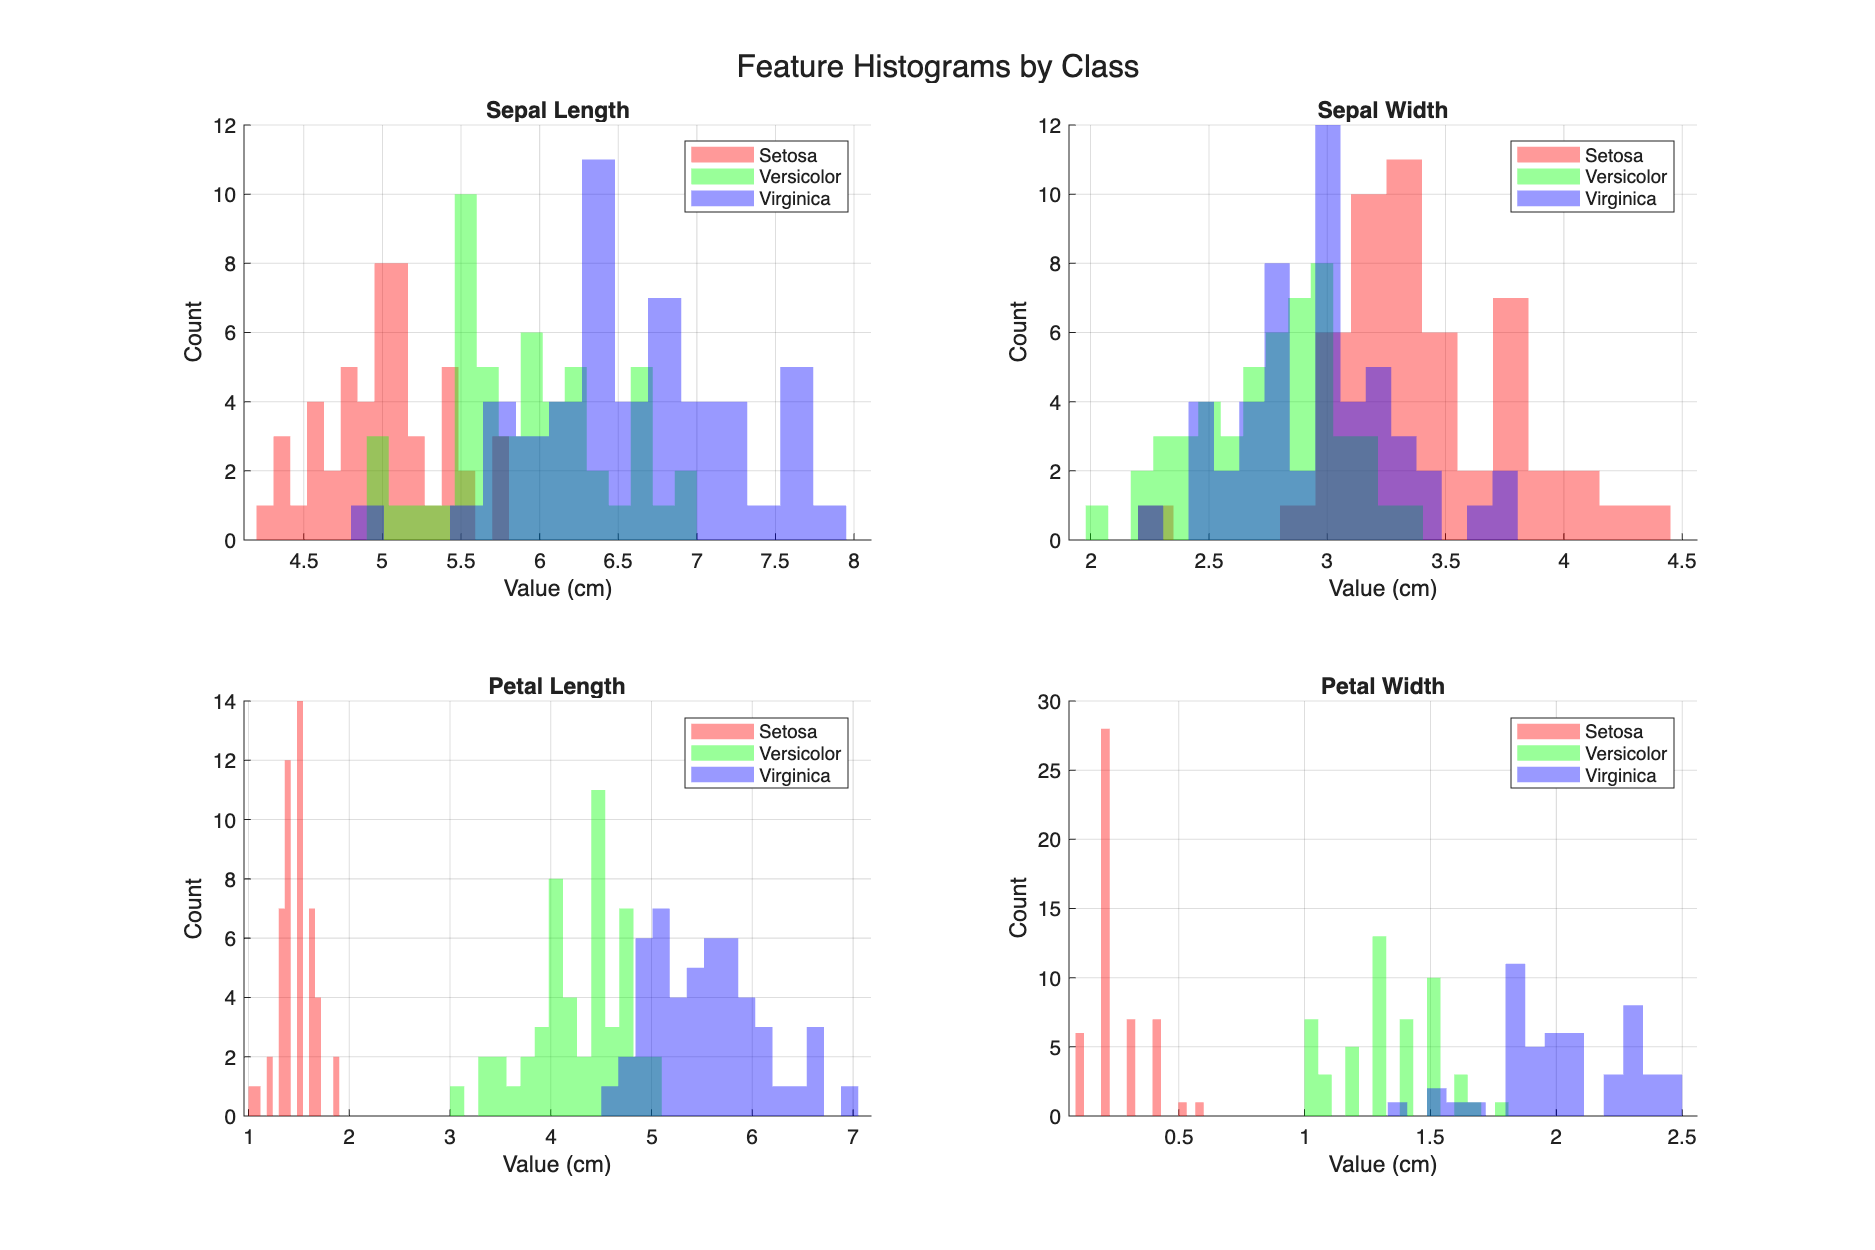
\includegraphics[width=0.9\textwidth]{feature_histograms.png}
\caption{Histograms of the four Iris features for each class. Setosa (red), Versicolor (green), Virginica (blue).}
\label{fig:histograms}
\end{figure}

To make the visual impression quantitative, we compute a histogram-based overlap score for each feature: for every pair of classes $(c_1,c_2)$ the histograms (normalized to unit area with 30 bins over the common range) are compared bin-by-bin by $\sum_b \min(h_{c_1}(b), h_{c_2}(b))$, and the three pairwise overlaps are summed. The scores obtained from the full dataset are
\begin{center}
\begin{tabular}{lc}
\toprule
Feature & Overlap score \\
\midrule
Sepal Length & 0.76 \\
Sepal Width  & 1.48 \\
Petal Length & 0.14 \\
Petal Width  & 0.12 \\
\bottomrule
\end{tabular}
\end{center}
Sepal Width has by far the largest overlap and is therefore removed first. Sepal Length is removed next, then Petal Length, leaving Petal Width as the single most discriminative feature.

\bigskip
\noindent\textbf{Error rates for reduced feature sets:}
\begin{center}
\begin{tabular}{llcc}
\toprule
Experiment & Features Used & Train Error & Test Error \\
\midrule
4 features & SL, SW, PL, PW                     & 3.33\,\% & 3.33\,\% \\
3 features & SL, PL, PW \ (removed SW)          & 3.33\,\% & 5.00\,\% \\
2 features & PL, PW     \ (removed SW, SL)      & 6.67\,\% & 5.00\,\% \\
1 feature  & PW         \ (removed SW, SL, PL)  & 4.44\,\% & 6.67\,\% \\
\bottomrule
\end{tabular}
\end{center}
\textit{(SL = Sepal Length, SW = Sepal Width, PL = Petal Length, PW = Petal Width)}

\bigskip
\noindent\textbf{Confusion matrices for the four experiments (rows: true, columns: predicted):}

\bigskip
\noindent\textbf{4 features --- test:}
\begin{center}\begin{tabular}{c|ccc}\toprule
 & Se & Ve & Vi \\ \midrule
Se & 20 & 0 & 0 \\
Ve & 0 & 18 & 2 \\
Vi & 0 & 0 & 20 \\
\bottomrule\end{tabular}\end{center}

\noindent\textbf{3 features --- test:}
\begin{center}\begin{tabular}{c|ccc}\toprule
 & Se & Ve & Vi \\ \midrule
Se & 20 & 0 & 0 \\
Ve & 0 & 18 & 2 \\
Vi & 0 & 1 & 19 \\
\bottomrule\end{tabular}\end{center}

\noindent\textbf{2 features --- test:}
\begin{center}\begin{tabular}{c|ccc}\toprule
 & Se & Ve & Vi \\ \midrule
Se & 20 & 0 & 0 \\
Ve & 0 & 19 & 1 \\
Vi & 0 & 2 & 18 \\
\bottomrule\end{tabular}\end{center}

\noindent\textbf{1 feature (PW) --- test:}
\begin{center}\begin{tabular}{c|ccc}\toprule
 & Se & Ve & Vi \\ \midrule
Se & 20 & 0 & 0 \\
Ve & 0 & 18 & 2 \\
Vi & 0 & 2 & 18 \\
\bottomrule\end{tabular}\end{center}

\bigskip
\textbf{Discussion.} The experiments confirm the feature ranking suggested by the histograms. Removing Sepal Width leaves the training error unchanged and raises the test error only slightly, confirming it as the weakest feature. Further removing Sepal Length actually gives the \emph{same} test error rate (5\,\%); because the two removed features carried mostly noise along the Versicolor--Virginica boundary, the gradient-descent solution simplifies without losing real information. With a single feature (Petal Width) the test error grows to 6.67\,\%, which is still remarkably low and demonstrates that Petal Width alone captures most of the class information.

Across all four experiments Setosa is classified without error, confirming that Setosa is linearly separable from the other two classes in \emph{every} non-trivial projection of the feature space. All errors arise at the Versicolor--Virginica boundary, which is a genuinely non-separable region. Two well-chosen petal features are therefore nearly sufficient for close-to-optimal linear classification of the Iris dataset, while the sepal measurements contribute comparatively little.

%% ======================================================================
\section{MNIST --- Implementation and Results}
\label{sec:mnist_results}
%% ======================================================================

This section describes the implementation and results of the handwritten-digit task. The MATLAB code is given in Appendix~\ref{app:mnist_code}.

\subsection{Implementation Overview}

The course-provided script \texttt{read09.m} is used once to read the four raw IDX files distributed with the MNIST database and store the result in \texttt{data\_all.mat}, which contains the variables \texttt{trainv} ($60\,000 \times 784$), \texttt{trainlab} ($60\,000 \times 1$), \texttt{testv} ($10\,000 \times 784$) and \texttt{testlab} ($10\,000 \times 1$). Because the feature dimension is high and the training set is large, the main efficiency concern is the $N_\text{test}\times N_T$ distance matrix. All our classifiers avoid forming it explicitly by
\begin{enumerate}
    \item casting \texttt{trainv} and \texttt{testv} to \texttt{double},
    \item pre-computing the row-wise squared norms $\|\mathbf{t}_j\|^2$ of the templates once, and
    \item evaluating squared distances chunk-by-chunk using Eq.~\eqref{eq:dist_trick}:
    the cross term $-2\,X T^T$ is one BLAS matrix multiplication per chunk, while the norm-sum is broadcast from cached vectors.
\end{enumerate}
With a chunk size of 1000 test images this brings memory use down to a manageable $1000\times60\,000$ matrix per iteration and exploits the heavy optimization of the linear-algebra routines.

\subsection{Task 1: NN Classifier with 60\,000 Templates}

\textbf{Classifier.} For each test image the nearest training image under Eq.~\eqref{eq:euclidean} is found and its label is returned (Eq.~\eqref{eq:nn}). The script \texttt{mnist\_task1.m} processes the test set in ten chunks of 1000 images and records, for every test image, the index of its nearest training neighbour so that misclassified and correctly classified samples can be displayed afterwards.

\textbf{Results.} Using all 60\,000 training vectors as templates, the classifier makes 309 errors on the 10\,000 test images, corresponding to an error rate of $3.09\,\%$. This matches the figure reported in the original MNIST benchmark for a plain NN classifier. The confusion matrix is shown in Table~\ref{tab:mnist_task1_conf}.

\begin{table}[ht]
\centering
\caption{Confusion matrix for the NN classifier using all 60\,000 training images as templates. Rows are the true class, columns the predicted class.}
\label{tab:mnist_task1_conf}
\small
\begin{tabular}{c|rrrrrrrrrr}
\toprule
 & 0 & 1 & 2 & 3 & 4 & 5 & 6 & 7 & 8 & 9 \\
\midrule
0 & 973 & 1 & 1 & 0 & 0 & 1 & 3 & 1 & 0 & 0 \\
1 & 0 & 1129 & 3 & 0 & 1 & 1 & 1 & 0 & 0 & 0 \\
2 & 7 & 6 & 992 & 5 & 1 & 0 & 2 & 16 & 3 & 0 \\
3 & 0 & 1 & 2 & 970 & 1 & 19 & 0 & 7 & 7 & 3 \\
4 & 0 & 7 & 0 & 0 & 944 & 0 & 3 & 5 & 1 & 22 \\
5 & 1 & 1 & 0 & 12 & 2 & 860 & 5 & 1 & 6 & 4 \\
6 & 4 & 2 & 0 & 0 & 3 & 5 & 944 & 0 & 0 & 0 \\
7 & 0 & 14 & 6 & 2 & 4 & 0 & 0 & 992 & 0 & 10 \\
8 & 6 & 1 & 3 & 14 & 5 & 13 & 3 & 4 & 920 & 5 \\
9 & 2 & 5 & 1 & 6 & 10 & 5 & 1 & 11 & 1 & 967 \\
\bottomrule
\end{tabular}
\end{table}

The most frequent confusions are the visually related pairs $3\leftrightarrow 5$ (19 errors), $4\to 9$ (22 errors), $8\to 3$ (14 errors) and $7\to 1$ (14 errors), all of which occur between digit shapes that differ only by a single stroke. Class~1 is classified almost perfectly (2 errors out of 1135, $99.47\,\%$ correct), while class~8 is the hardest (55 errors out of 974, $94.46\,\%$ correct).

\textbf{Runtime.} On our test machine the chunked classifier processes all 10\,000 test images in a few seconds with the BLAS-accelerated matrix product. The MATLAB implementation is typically somewhat slower than NumPy on the same hardware but remains well below one minute.

\textbf{Misclassified and correct examples.} Figure~\ref{fig:mnist_wrong} shows eight test images misclassified by the NN classifier. Several of them are ambiguous even to a human observer: for example an 8 whose lower loop has been closed into the shape of a 3, or a 7 drawn with a very short horizontal stroke which the classifier reads as a 1. Figure~\ref{fig:mnist_right} shows eight correctly classified images; these are clean, canonical-looking digits for which the nearest training example is easy to find.

\begin{figure}[ht]
\centering
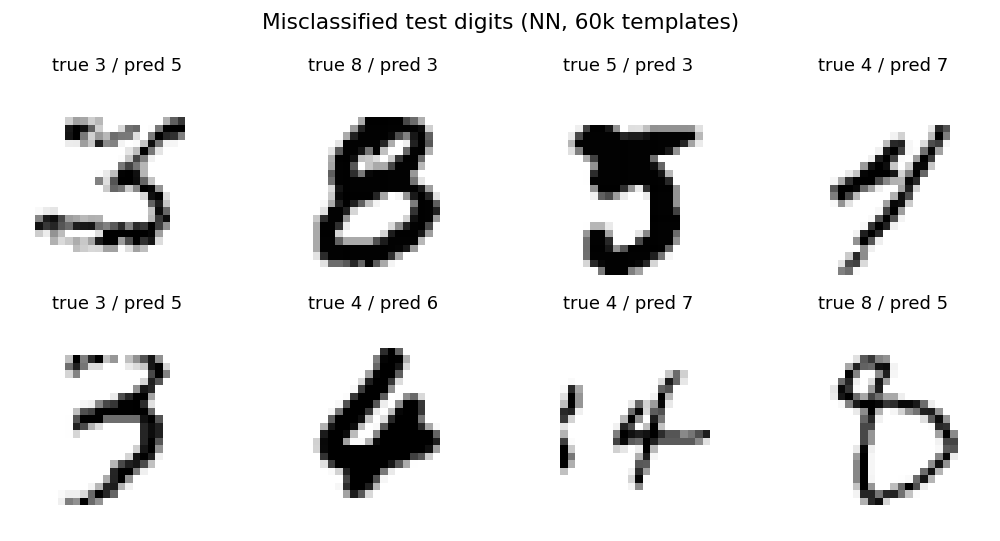
\includegraphics[width=0.95\textwidth]{mnist_misclassified.png}
\caption{Eight test images misclassified by the NN classifier trained on all 60\,000 MNIST templates. Titles give the true label and the prediction.}
\label{fig:mnist_wrong}
\end{figure}

\begin{figure}[ht]
\centering
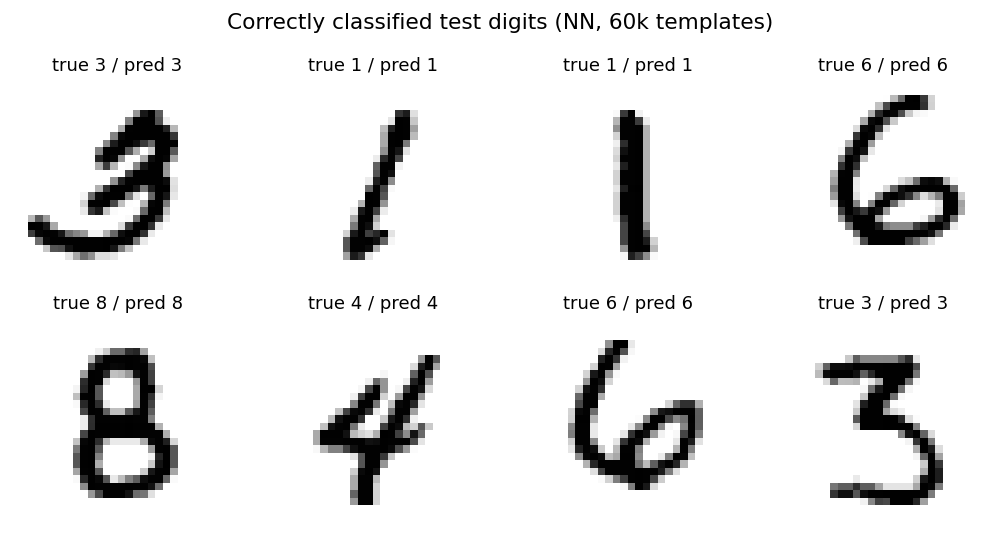
\includegraphics[width=0.95\textwidth]{mnist_correct.png}
\caption{Eight test images correctly classified by the NN classifier.}
\label{fig:mnist_right}
\end{figure}

\subsection{Task 2: Clustered Templates, NN and KNN}

\textbf{Clustering.} The 60\,000 training vectors are split by class (about 6000 per class) and the MATLAB function \texttt{kmeans} is called once per class with $M=64$ clusters. The returned 64 centroids for class~$i$ are stacked into a template matrix $C\in\mathbb{R}^{640\times 784}$ with an accompanying label vector $c\in\{0,\dots,9\}^{640}$. Figure~\ref{fig:mnist_templates} displays 8 of the 64 templates for every class; they closely resemble average handwritten digits, which is expected since a cluster centroid is the mean of the training vectors in that cluster.

\begin{figure}[ht]
\centering
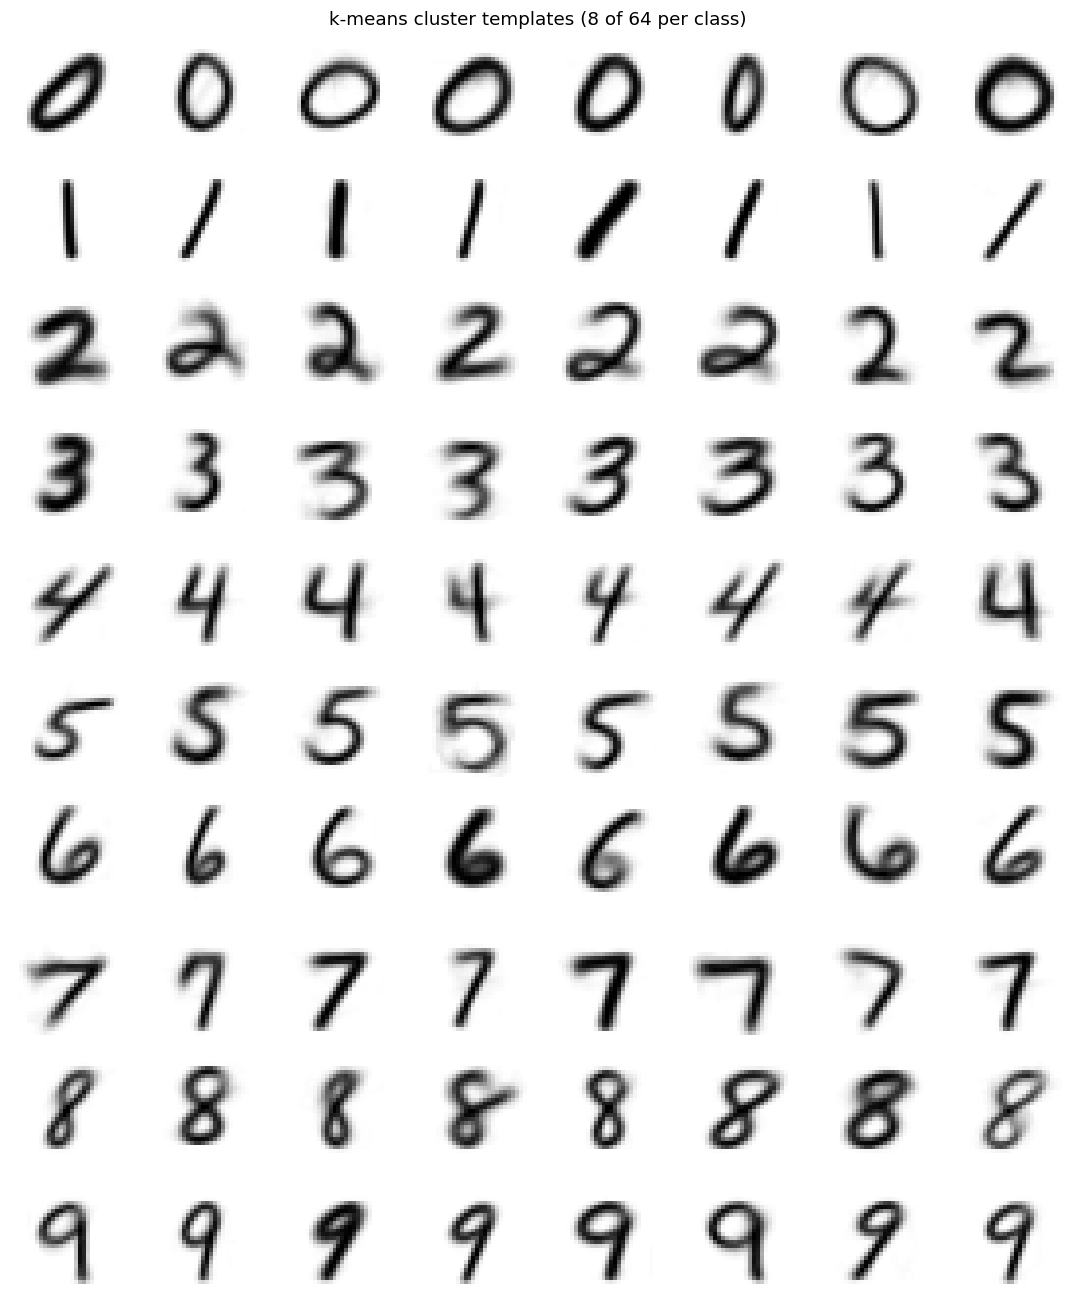
\includegraphics[width=0.85\textwidth]{mnist_cluster_templates.png}
\caption{Eight of the 64 $k$-means cluster templates per digit class. Each row corresponds to one class 0--9.}
\label{fig:mnist_templates}
\end{figure}

\textbf{NN on 640 templates.} The 1-NN classifier of Eq.~\eqref{eq:nn} is then run against the 640 clustered templates. The entire $10\,000\times 640$ distance matrix can be formed in one shot. The error rate rises to $4.78\,\%$ (478 errors out of 10\,000), as shown in Table~\ref{tab:mnist_task2_nn_conf}. The classification time drops drastically: the dominant cost of the full-template classifier is the $10\,000\times 60\,000$ matrix product, whereas the clustered classifier requires only a $10\,000\times 640$ product---about a hundredfold speed-up. Taking the one-time clustering cost into account, the clustered classifier pays for itself as soon as the same template set is reused across several test runs.

\begin{table}[ht]
\centering
\caption{Confusion matrix for the 1-NN classifier with 640 clustered templates.}
\label{tab:mnist_task2_nn_conf}
\small
\begin{tabular}{c|rrrrrrrrrr}
\toprule
 & 0 & 1 & 2 & 3 & 4 & 5 & 6 & 7 & 8 & 9 \\
\midrule
0 & 966 & 1 & 3 & 1 & 0 & 4 & 3 & 1 & 0 & 1 \\
1 & 0 & 1126 & 3 & 1 & 0 & 0 & 3 & 0 & 1 & 1 \\
2 & 9 & 8 & 979 & 8 & 1 & 0 & 3 & 11 & 12 & 1 \\
3 & 0 & 0 & 7 & 940 & 1 & 32 & 0 & 6 & 17 & 7 \\
4 & 1 & 6 & 2 & 0 & 922 & 0 & 10 & 4 & 3 & 34 \\
5 & 3 & 1 & 0 & 20 & 2 & 845 & 9 & 1 & 7 & 4 \\
6 & 9 & 3 & 2 & 0 & 3 & 3 & 934 & 0 & 3 & 1 \\
7 & 0 & 20 & 8 & 0 & 4 & 1 & 0 & 961 & 2 & 32 \\
8 & 5 & 1 & 3 & 11 & 3 & 20 & 2 & 6 & 917 & 6 \\
9 & 5 & 6 & 4 & 5 & 30 & 1 & 1 & 19 & 6 & 932 \\
\bottomrule
\end{tabular}
\end{table}

\textbf{KNN with $K=7$.} The same 640 templates are used by a KNN classifier (Eq.~\eqref{eq:knn}) with $K=7$. For every test image the seven closest templates are found with \texttt{sort} and a majority vote is taken with \texttt{mode}. The error rate is $6.31\,\%$ (631 errors), see Table~\ref{tab:mnist_task2_knn_conf}.

\begin{table}[ht]
\centering
\caption{Confusion matrix for the KNN classifier ($K=7$) on the 640 cluster templates.}
\label{tab:mnist_task2_knn_conf}
\small
\begin{tabular}{c|rrrrrrrrrr}
\toprule
 & 0 & 1 & 2 & 3 & 4 & 5 & 6 & 7 & 8 & 9 \\
\midrule
0 & 952 & 1 & 3 & 0 & 0 & 8 & 13 & 1 & 2 & 0 \\
1 & 0 & 1128 & 2 & 1 & 0 & 1 & 2 & 0 & 1 & 0 \\
2 & 13 & 15 & 952 & 12 & 3 & 1 & 4 & 14 & 18 & 0 \\
3 & 2 & 3 & 8 & 947 & 2 & 19 & 0 & 12 & 14 & 3 \\
4 & 1 & 14 & 4 & 0 & 901 & 0 & 7 & 2 & 2 & 51 \\
5 & 3 & 3 & 4 & 28 & 4 & 836 & 7 & 1 & 4 & 2 \\
6 & 10 & 4 & 4 & 0 & 5 & 10 & 923 & 0 & 2 & 0 \\
7 & 0 & 33 & 13 & 2 & 12 & 0 & 0 & 939 & 0 & 29 \\
8 & 5 & 3 & 6 & 25 & 10 & 32 & 2 & 7 & 875 & 9 \\
9 & 7 & 9 & 3 & 9 & 32 & 4 & 1 & 20 & 8 & 916 \\
\bottomrule
\end{tabular}
\end{table}

\subsection{Comparison of the Three Systems}

\begin{center}
\begin{tabular}{lccc}
\toprule
System & \#~templates & Error rate & Relative classification time \\
\midrule
NN, full training set   & 60\,000 & 3.09\,\% & 1.0$\times$ (baseline) \\
NN, clustered templates &    640 & 4.78\,\% & $\approx 0.01\times$ \\
KNN, $K=7$, clustered    &    640 & 6.31\,\% & $\approx 0.03\times$ \\
\bottomrule
\end{tabular}
\end{center}

\textbf{Discussion.} The full-template NN classifier is the most accurate of the three, because every idiosyncratic handwriting style in the test set has a chance of matching an actual training image. Replacing the 60\,000 real images with 640 cluster centroids loses the long tail of unusual handwriting and costs about 1.7 percentage points of accuracy---but buys roughly two orders of magnitude in classification time. For $K=7$ on the small template set the accuracy drops another 1.5 percentage points: with only 64 templates per class, the seven nearest templates frequently have to stretch across more than one ``visual cluster'' of the class, and the majority vote dilutes the local evidence that the 1-NN rule captures so well. Consistent with this, the per-class accuracy drops most for classes with intrinsically diverse handwriting---most notably class~4 ($9$ being a frequent competitor) and class~5.

In summary, the full-training-set NN is the accuracy ceiling among the three compendium-style NN classifiers for MNIST, while the clustered 1-NN classifier gives the best speed/accuracy trade-off; the $K=7$ variant does not help here because the template set is too small for a majority vote to outperform the single nearest centroid.

%% ======================================================================
\section{Conclusion}
\label{sec:conclusion}
%% ======================================================================

In the \emph{Iris} part of this project a linear MSE classifier was implemented in MATLAB following exactly the formulation of chapters~2.4 and~3.2 of the compendium: linear discriminant (Eq.~7), sigmoid activation (Eq.~20), MSE cost (Eq.~19), gradient (Eq.~22) and weight update (Eq.~23). The classifier was trained using batch gradient descent with a step factor $\alpha = 0.005$ over $M = 3000$ iterations, which produced smooth monotone convergence of the MSE.

The first Iris experiment showed that the classifier achieves low error rates on the Iris dataset. In Case~1 the training and test error are identical at $3.33\,\%$; in Case~2 the training error is $5.56\,\%$ while the test error is $0\,\%$. All misclassifications occur at the Versicolor--Virginica boundary, while Setosa is always perfectly classified. The difference between the two cases reflects the ordering of the samples in the provided files rather than any asymmetry of the classifier. The second experiment demonstrated that the four features contribute unequally: the petal features are by far the most discriminative, and a single-feature classifier based on petal width still achieves a $6.67\,\%$ test error.

In the \emph{MNIST} part, the nearest-neighbour classifiers of chapter~3 were implemented with chunked Euclidean-distance computation. Using the full 60\,000-image training set as templates yields an error rate of $3.09\,\%$, which matches the reference number for plain NN on MNIST. Clustering each class into $M=64$ prototypes with $k$-means produces a 640-template classifier that is roughly two orders of magnitude faster to evaluate and still achieves $4.78\,\%$ error. A $K=7$ KNN classifier on the same 640 templates degrades slightly to $6.31\,\%$ because the template set is too small for a majority vote to beat the single nearest centroid. Across all three systems the most frequent confusions are between visually similar digit pairs (e.g.\ $3\leftrightarrow 5$ and $4\leftrightarrow 9$), exactly as expected.

The project provided practical experience with implementing and evaluating two of the fundamental classifier families in the compendium---a gradient-descent-trained linear classifier and distance-based nearest-neighbour classifiers---and with the classical speed/accuracy trade-offs introduced by template clustering.

%% ======================================================================
\begin{thebibliography}{9}
\bibitem{fisher1936}
R.~A.~Fisher, ``The use of multiple measurements in taxonomic problems,'' \textit{Annals of Eugenics}, vol.~7, no.~2, pp.~179--188, 1936.

\bibitem{compendium}
TTT4275 Compendium --- Part III --- Classification, NTNU, 2025.

\bibitem{irisdata}
Iris flower data set, \url{https://en.wikipedia.org/wiki/Iris_flower_data_set}.
\end{thebibliography}

%% ======================================================================
\appendix

\section{MATLAB Code --- Iris}
\label{app:iris_code}

\subsection{Task 1: Training and Generalization}
\lstinputlisting[style=matlab, caption={iris\_task1.m}]{iris_task1.m}

\subsection{Task 2: Features and Linear Separability}
\lstinputlisting[style=matlab, caption={iris\_task2.m}]{iris_task2.m}

\section{MATLAB Code --- MNIST}
\label{app:mnist_code}

\subsection{Task 1: NN classifier with the full training set}
\lstinputlisting[style=matlab, caption={mnist\_task1.m}]{mnist_task1.m}

\subsection{Task 2: Clustered templates, NN and KNN}
\lstinputlisting[style=matlab, caption={mnist\_task2.m}]{mnist_task2.m}

\end{document}
